\documentclass[]{article}
\usepackage{lmodern}
\usepackage{amssymb,amsmath}
\usepackage{ifxetex,ifluatex}
\usepackage{fixltx2e} % provides \textsubscript
\ifnum 0\ifxetex 1\fi\ifluatex 1\fi=0 % if pdftex
  \usepackage[T1]{fontenc}
  \usepackage[utf8]{inputenc}
\else % if luatex or xelatex
  \ifxetex
    \usepackage{mathspec}
    \usepackage{xltxtra,xunicode}
  \else
    \usepackage{fontspec}
  \fi
  \defaultfontfeatures{Mapping=tex-text,Scale=MatchLowercase}
  \newcommand{\euro}{€}
\fi
% use upquote if available, for straight quotes in verbatim environments
\IfFileExists{upquote.sty}{\usepackage{upquote}}{}
% use microtype if available
\IfFileExists{microtype.sty}{%
\usepackage{microtype}
\UseMicrotypeSet[protrusion]{basicmath} % disable protrusion for tt fonts
}{}
\usepackage[margin=1in]{geometry}
\usepackage{longtable,booktabs}
\usepackage{graphicx}
\makeatletter
\def\maxwidth{\ifdim\Gin@nat@width>\linewidth\linewidth\else\Gin@nat@width\fi}
\def\maxheight{\ifdim\Gin@nat@height>\textheight\textheight\else\Gin@nat@height\fi}
\makeatother
% Scale images if necessary, so that they will not overflow the page
% margins by default, and it is still possible to overwrite the defaults
% using explicit options in \includegraphics[width, height, ...]{}
\setkeys{Gin}{width=\maxwidth,height=\maxheight,keepaspectratio}
\ifxetex
  \usepackage[setpagesize=false, % page size defined by xetex
              unicode=false, % unicode breaks when used with xetex
              xetex]{hyperref}
\else
  \usepackage[unicode=true]{hyperref}
\fi
\hypersetup{breaklinks=true,
            bookmarks=true,
            pdfauthor={Innocence Harvey and Dave Bridges},
            pdftitle={Post High Protein Diet CLAMS},
            colorlinks=true,
            citecolor=blue,
            urlcolor=blue,
            linkcolor=magenta,
            pdfborder={0 0 0}}
\urlstyle{same}  % don't use monospace font for urls
\setlength{\parindent}{0pt}
\setlength{\parskip}{6pt plus 2pt minus 1pt}
\setlength{\emergencystretch}{3em}  % prevent overfull lines
\setcounter{secnumdepth}{0}

%%% Use protect on footnotes to avoid problems with footnotes in titles
\let\rmarkdownfootnote\footnote%
\def\footnote{\protect\rmarkdownfootnote}

%%% Change title format to be more compact
\usepackage{titling}

% Create subtitle command for use in maketitle
\newcommand{\subtitle}[1]{
  \posttitle{
    \begin{center}\large#1\end{center}
    }
}

\setlength{\droptitle}{-2em}
  \title{Post High Protein Diet CLAMS}
  \pretitle{\vspace{\droptitle}\centering\huge}
  \posttitle{\par}
  \author{Innocence Harvey and Dave Bridges}
  \preauthor{\centering\large\emph}
  \postauthor{\par}
  \predate{\centering\large\emph}
  \postdate{\par}
  \date{May 29, 2015}



\begin{document}

\maketitle


The input files were CLAMS MRI Data.xlsx for the echoMRI data. This
script was most recently updated on Tue Sep 8 15:20:29 2015 and includes
the following number of animals.

The following animals/data were removed from this analysis due to data
that was either not collected (ie measurements after the run was
complete) or data that was clearly incorrect (airflow problems):

\begin{longtable}[c]{@{}lr@{}}
\toprule
Treatment & Males\tabularnewline
\midrule
\endhead
Control Diet & 6\tabularnewline
High Protein Diet & 6\tabularnewline
\bottomrule
\end{longtable}

\section{Resting Metabolic Rate}\label{resting-metabolic-rate}

The VO2 levels were first merged to average over light and dark cycles,
removing the first 20 measurements. To analyse these data we performed
an ANCOVA analysis using lean body mass as the primary covariate.

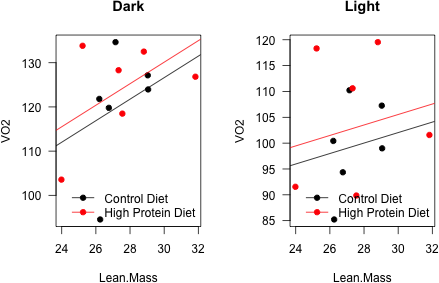
\includegraphics{figures/VO2-by-lean-1.png}

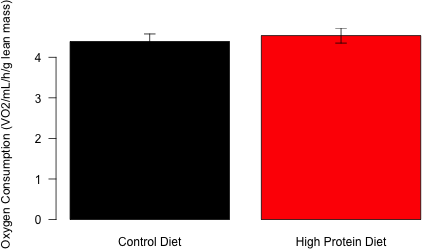
\includegraphics{figures/vo2-barplot-1.png}

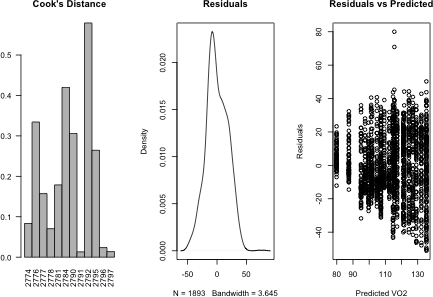
\includegraphics{figures/vo2-diagnostic-plots-1.png}

We first checked whether normality was maintained in the residuals from
the ANCOVA. These results are summarized below:

\begin{longtable}[c]{@{}lrrrrr@{}}
\caption{ANCOVA Analysis for Effect of Diet on VO2}\tabularnewline
\toprule
& Df & Sum Sq & Mean Sq & F value & Pr(\textgreater{}F)\tabularnewline
\midrule
\endfirsthead
\toprule
& Df & Sum Sq & Mean Sq & F value & Pr(\textgreater{}F)\tabularnewline
\midrule
\endhead
Lean.Mass & 1 & 282.1 & 282.1 & 2.208 & 0.1529\tabularnewline
Light.Dark & 1 & 2349.4 & 2349.4 & 18.390 & 0.0004\tabularnewline
Treatment & 1 & 129.2 & 129.2 & 1.011 & 0.3266\tabularnewline
Residuals & 20 & 2555.2 & 127.8 & NA & NA\tabularnewline
\bottomrule
\end{longtable}

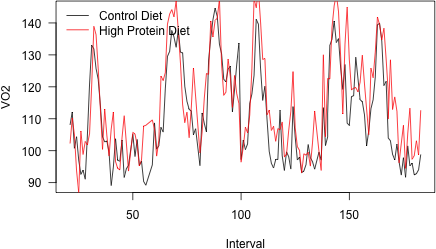
\includegraphics{figures/vo2-time-course-1.png}

The residuals of this model were normally distributed (p=0.7224) via a
Shapiro-Wilk Test. According to this ANCOVA, the double knockouts have
4.6407 higher VO2, a reduction of 3.7357\%

Alternatively we used a mixed linear model, with non-interacting
covariates for the Light cycle, the lean mass and the diet. A
Chi-squared test comparing a model with or without the Diet term yielded
a p-value of 0.4337 for the males. The residuals of this model were
\textbf{not normally distributed} ( via Shapiro-Wilk Test).

\section{Body Weights and
Composition}\label{body-weights-and-composition}

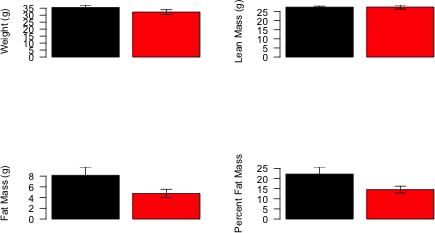
\includegraphics{figures/body-composition-no-treatment-1.png}

\begin{longtable}[c]{@{}lrrrrr@{}}
\caption{Statistical Tests for Body Composition}\tabularnewline
\toprule
& Shapiro & Levene & Wilcox & Welch & Student\tabularnewline
\midrule
\endfirsthead
\toprule
& Shapiro & Levene & Wilcox & Welch & Student\tabularnewline
\midrule
\endhead
Body Weight & 0.4481 & 0.9653 & 0.2403 & 0.1847 & 0.1845\tabularnewline
Fat Mass & 0.4432 & 0.0769 & 0.1320 & 0.0906 & 0.0795\tabularnewline
Percent Fat Mass & 0.2101 & 0.1054 & 0.1320 & 0.0873 &
0.0762\tabularnewline
Lean Mass & 0.0768 & 0.2695 & 1.0000 & 0.9733 & 0.9730\tabularnewline
\bottomrule
\end{longtable}

\section{Respiratory Exchange Rate}\label{respiratory-exchange-rate}

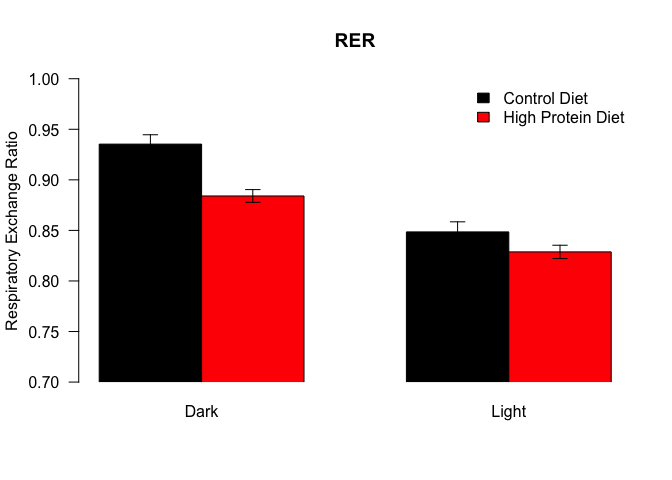
\includegraphics{figures/rer-barplot-1.png}

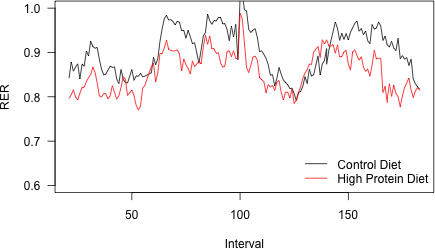
\includegraphics{figures/rer-time-course-1.png}

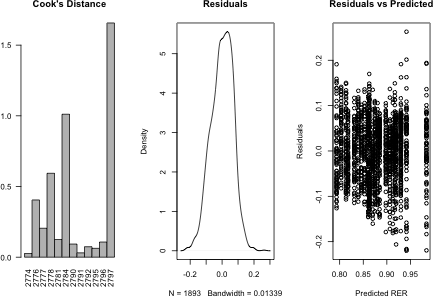
\includegraphics{figures/rer-statistics-untreated-1.png}

Alternatively we used a mixed linear model, with non-interacting
covariates for the Light cycle and the diet. A Chi-squared test
comparing a model with or without the diet term yielded a p-value of
0.0038 for the males.

\section{Activity Data}\label{activity-data}

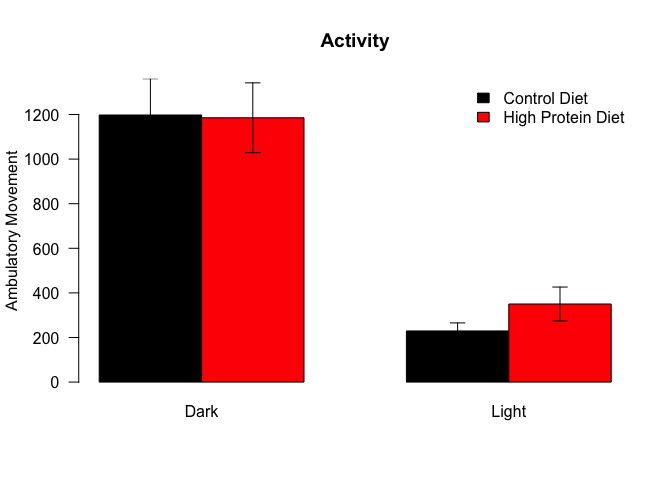
\includegraphics{figures/activity-1.png}

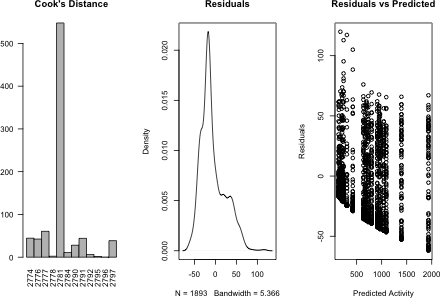
\includegraphics{figures/activity-statistics-1.png}

Alternatively we used a mixed linear model, with non-interacting
covariates for the Light cycle and the diet. A Chi-squared test
comparing a model with or without the Genotype term yielded a p-value of
0.5042 for the males.

\section{Session Information}\label{session-information}

\begin{verbatim}
## R version 3.2.2 (2015-08-14)
## Platform: x86_64-apple-darwin13.4.0 (64-bit)
## Running under: OS X 10.10.4 (Yosemite)
## 
## locale:
## [1] en_US.UTF-8/en_US.UTF-8/en_US.UTF-8/C/en_US.UTF-8/en_US.UTF-8
## 
## attached base packages:
## [1] stats     graphics  grDevices utils     datasets  methods   base     
## 
## other attached packages:
##  [1] tidyr_0.2.0        car_2.0-26         influence.ME_0.9-6
##  [4] lme4_1.1-8         Matrix_1.2-2       reshape2_1.4.1    
##  [7] xtable_1.7-4       lubridate_1.3.3    dplyr_0.4.2       
## [10] xlsx_0.5.7         xlsxjars_0.6.1     rJava_0.9-7       
## [13] knitr_1.11        
## 
## loaded via a namespace (and not attached):
##  [1] Rcpp_0.12.0     formatR_1.2     nloptr_1.0.4    plyr_1.8.3     
##  [5] highr_0.5       tools_3.2.2     digest_0.6.8    evaluate_0.7.2 
##  [9] memoise_0.2.1   nlme_3.1-121    lattice_0.20-33 mgcv_1.8-7     
## [13] DBI_0.3.1       yaml_2.1.13     parallel_3.2.2  SparseM_1.7    
## [17] stringr_1.0.0   grid_3.2.2      nnet_7.3-10     R6_2.1.1       
## [21] rmarkdown_0.7   minqa_1.2.4     magrittr_1.5    htmltools_0.2.6
## [25] splines_3.2.2   MASS_7.3-43     assertthat_0.1  pbkrtest_0.4-2 
## [29] quantreg_5.11   stringi_0.5-5   lazyeval_0.1.10
\end{verbatim}

\end{document}
